\documentclass{article}
\title{Machine Learning Notes}
\date{2022}
\author{João Rocha}
	
\usepackage[utf8]{inputenc}
\usepackage{hyperref}
\usepackage{indentfirst}
\usepackage{comment}
\usepackage{amsmath}
\usepackage{bbm}
\usepackage{amssymb}
\usepackage{mathtools, nccmath}
\usepackage{geometry}
\usepackage{subcaption}
\usepackage{graphicx}

\geometry{
    a4paper,
    total={129mm,170mm},
    left=23mm,
    top=23mm,
    bottom=28mm,
    right=28mm,
}

\newcommand{\R}{\mathbb{R}}
\newcommand{\N}{\mathbb{N}}
\newcommand{\Z}{\mathbb{Z}}
\newcommand{\C}{\mathbb{C}}
\newcommand{\prob}{\mathbb{P}}
\newcommand{\E}{\mathbb{E}}
\newcommand{\var}{\mathbb{V}}
\newcommand{\ind}{\mathbbm{1}}
\newcommand{\indep}{\perp \!\!\! \perp}
\newcommand{\loss}{\mathcal{L}}
\newcommand{\dist}{\mathcal{D}}

\begin{document}
\maketitle
\tableofcontents
\vspace*{\fill}
\textbf{WARNING}:\\ 
This text is essentially a summary of some essential knowledge in Machine Learning and does not aim to go into detailed explanations of the concepts covered.
The main objective of this document is hence to be a reference, and not to clarify.
However, some topics are accompanied by brief explanations, in order to remind the intuition behind them.\\
This text was made by the author while in preparation for both its Bachelor Machine Learning course at Instituto Superior Técnico @ Lisbon, Portugal and its Master Machine Learning course at EPFL @ Lausanne, Switzerland, also with some consultation of Stanford's online content.
Be advised that the content does not coincide exactly with neither of these courses and may be presented in different fashion from them.\\
Contributions, corrections and suggestions are welcome at \href{https://github.com/Calhau18/Machine_Learning_Notes}{the document's repo}.
\newpage

\section{Introduction}

Traditional algorithms encompass a set of rules that, given some data, determine some output.
On certain problems, however, it is hard to determine the set of rules that produce a given output.
We would hence like to produce algorithms with the capacity of inferring a set of rules that can produce some output given some data.
Machine Learning encompasses techniques for inferring these rules (we "train" the model) that can then be used to deduce the outputs on unseen data (i.e, perform "predictions").

Usually, learning in Machine Learning consists in choosing some model that is based on a certain set of \textbf{assumptions} and has some \textbf{parameters} that are tuned for the given data.
As such, most Machine Learning predictors can be mathematically defined as functions $f : \mathcal{X} \times \Theta \to \mathcal{Y}$ where $\mathcal{X}$ is a set of possible inputs, $\Theta$ the set of parameters of the model and $\mathcal{Y}$ an output set.
We will denote $f(x ; \theta)$ for the value of the predictor with parameters $\theta$ on an input $x$.

The process of training a model can also be seen as a function $\mathcal{A} : D \times \mathcal{H} \to \Theta$ that infers a set of prediction parameters $\theta \in \Theta$ from a set of training parameters $\eta \in \mathcal{H}$ and a training dataset $D$ drawn from some data distribution $\mathcal{D}$.
Mathematically, we usually want these parameters to maximize the quality of the model / minimize the amount of errors the model make.
As such, training a Machine Learning model is usually formalized as finding the solution to  the following minimization problem:
$$
\min_{\theta \in \Theta} \E_{x \sim \mathcal{D}} \left[ \loss(x) \right]
$$
where $\loss$ is called a \textbf{loss / error / cost function}.

\subsection{Loss Functions}

There are a few properties that are usually desirable from loss functions:
\begin{itemize}
    \item When the target $y$ is real-valued, it is often desirable that the cost is symmetric around 0, since both positive and negative errors should be penalized equally;
    \item Penalize large mistakes similarly to very large mistakes, i.e, be robust to outliers;
    \item Have properties that make it easy to minimize computationally, namely \textbf{convexity} and \textbf{differentiability} (or at least allow a subgradient).
\end{itemize}

Some common loss functions are:
\begin{itemize}
    \item \textbf{Mean Squared Error}: 
	$\loss(y, \hat{y}) = \frac{1}{N} ||y - \hat{y}||_2^2 = \frac{1}{N} \sum_{i=1}^N (y_i - \hat{y}_i)^2$\\
	Very common loss function but not very robust to outliers. Differentiable and convex.
    \item \textbf{Mean Absolute Error}: 
	$\loss(y, \hat{y}) = \frac{1}{N} ||y - \hat{y}||_1 = \frac{1}{N} \sum_{i=1}^N |y_i - \hat{y}_i|$\\
	More robust to outliers but not differentiable. It accepts however a subgradient.
	\item \textbf{Logistic Loss}:
	$\loss(y, \hat{y}) = \frac{1}{N} \sum_{i=1}^N \log(1 + e^{-y_i \hat{y}_i})$\\
	Used for classification problems. Differentiable and convex.
	\item \textbf{Hinge Loss}:
	$\loss(y, \hat{y}) = \frac{1}{N} \sum_{i=1}^N \max(0, 1 - y_i \hat{y}_i)$\\
	Used for classification problems. Differentiable and convex.
\end{itemize}

\subsection{Optimization}

As learning problems are usually formalized as minimization problems, we can use normal optimization techniques to solve them.

\subsubsection{Grid Search}

Grid search is one of the simplest optimization algorithms. 
We compute the cost over all values w in a grid, and pick the best among those.

This is brute-force, but extremely simple and works for any kind of cost function when we have very few parameters and the cost is easy to compute.

However, for a large number of parameters, grid-search results in an exponential computational complexity.
Moreover, grid search provides no analytic method to find an optimum - it only selects the best value from a set of hypothesis.

Grid search is most frequently used for hyperparameter tuning, i.e, to select the best hyperparameters of a model from a set of reasonable hypothesis.
As these hyperparameter selections are often independent, this computation is very well parallelizable.

\subsubsection{Gradient Descent} 

Gradient Descent arises from the idea that moving in the direction of $-\nabla f$ always decreases the value of $f$ (for a sufficiently small "step").
Therefore, the gradient descent algorithm can be briefly described as follows:
\begin{enumerate}
    \item Choose a starting point $x^{(0)} \in \mathcal{X}$.
    \item Repeat until convergence:
    \begin{enumerate}
	\item Compute $x^{(k+1)} = x^{(k)} - \gamma \nabla f(x^{(k)})$, for a \textbf{learning rate} $\gamma \in \R^+$.
    \end{enumerate}
\end{enumerate}

This algorithm is guaranteed to converge to a \textit{local minimum} of $f$.
Therefore, in the case of strictly convex functions, it will converge to the global minimum, as strictly convex functions have a unique (global) minimum.

Note that the computation of this algorithm can be expensive. 
For example, both in linear and logistic regression, the computation of the gradient takes $O(DN)$ time.
We perform this computation once per update.
Defining $s$ as the number of gradient descent steps until convergence, the complexity of the algorithm is $O(DNs)$.

\paragraph{Learning Rate}
The value of $s$ depends strongly on the choice of $\gamma$.
If $\gamma$ is too small, the algorithm will take a long time to converge.
However, setting $\gamma$ to a larger number might cause the algorithm to "overshoot" the intended minimum, stopping it from converging.
The choice of $\gamma$ is therefore a delicate balance, and it is usually chosen by trial and error.
A frequent option is to start with a large $\gamma$ and decrease it as the algorithm converges.
The algorithm is always guaranteed to converge for $\gamma < \gamma_{\min}$, where the value of $\gamma_{\min}$ is dependent on the problem.

\paragraph{}
It should also be noted that the computation of a gradient is easily parallelizable as its computation is independent in each entry point.

Finally, gradient descent is very sensitive to ill-conditioning.
Therefore, it is typically advised to normalize your input features.
In other words, we pre-condition the optimization problem.
Without this, step-size selection is more difficult since different “directions” might converge at different speed.

\subsubsection{Stochastic Gradient Descent} 

SGD is a variation of the gradient descent algorithm that addresses the problem that computing a gradient may be expensive for a big dataset.
SGD thus works by selecting only a single entry at a time and moving in the direction of its gradient.  

Since, in expectation, the gradient of a single entry is the same as the gradient of the whole dataset, this algorithm is expected to move in the correct direction over a reasonable amount of steps.  

However, performing a single step is $N$ times faster than true GD, as we only have to analyze a single entry.
Depending on the effect this has on the number of steps $s$ required to converge, this can allow a great reduction in execution time.

\subsubsection{Batch Gradient Descent} 

BGD is a compromise between the accuracy of descent of traditional GD and the smaller computation cost of SGD. 
This algorithm samples $B$ entries from the dataset and computes the gradient of the loss function over these entries.

As such, and while the expectation of the gradient direction is the same as true GD, the variation of this direction is much smaller ($B$ times smaller) than that of SGD.
The sacrifice is that it also takes $B$ times longer to compute a batch gradient than a stochastic gradient.
Once again, depending on convergence speed, this can be a good compromise.

\subsubsection{Subgradient Descent}

The idea of gradient descent is only applicable to differentiable functions, as it requires that a gradient can be computed.
For differentiable functions, convexity can be expressed as
$$
f(u) \geq f(w) + \nabla f(w)^T (u-w) \ \forall u,w
$$

The idea of a subgradient generalizes this expression.
A vector $g \in \R^D$ is such that
$$
f(u) \geq f(w) + g^T (u - w) \ \forall u
$$
is said to be a subgradient of $f$ at $w$.

For a subgradient function $g(w): \R^n \to \R^n$, we can adapt the Gradient Descent algorithms (true, stochastic, and batch) to SubGradient Descent algorithms by following the direction of $-g$ instead of $-\nabla f$.

Subgradient descent is guaranteed to converge to a global minima.

\subsubsection{Variants of SGD}

\paragraph{Momentum}

Momentum works by adding a momentum term to the update rule, which is a weighted average of the previous updates.

\begin{gather*}
m^{(t+1)} = \beta m^{(t)} + (1 - \beta)g \\
w^{(t+1)} = w^{(t)} - \gamma m^{(t+1)}
\end{gather*}

\paragraph{Adagrad}

Adagrad is a technique that decreases the learning rate over time according to the size of the gradients.
$$
w^{(t+1)} = w^{(t)} - \frac{\gamma}{\sqrt{\sum_{i=0}^t \nabla f(w^{(i)})^2}} \nabla f(w^{(t)})
$$

\paragraph{RMSProp}

RMSProp is a variation of Adagrad that improves convergence speed by taking into account only the most recent gradients.

$$
w^{(t+1)} = w^{(t)} - \frac{\gamma}{\sqrt{\sum_{i=t-k}^t \nabla f(w^{(i)})^2}} \nabla f(w^{(t)})
$$

\paragraph{Adam}

Adam combines the idea of RMSProp and momentum.

\begin{gather*}
m^{(t+1)} = \beta_1 m^{(t)} + (1 - \beta_1)g \\
v_i^{(t+1)} = \beta_2 v_i^{(t)} + (1 - \beta_2) g_i^2 \ \forall i \\
w_i^{(t+1)} = w_i^{(t)} - \frac{\gamma}{\sqrt{v_i^{(t+1)}}} m_i^{(t+1)} \ \forall i
\end{gather*}

\paragraph{SignSGD}

SignSGD only uses the sign (one bit) of each gradient allowing more efficient communication for distributed training. 
It has however convergence issues

$$
w_i^{(t+1)} = w_i^{(t)} - \gamma \text{sign}(g_i) \ \forall i
$$

\subsubsection{Constrained Optimization}

Sometimes, optimization problems come posed with additional constraints:

$$
\min_{w} \loss(w) \quad \text{s.t.} \ w \in \mathcal{C}
$$

where $\mathcal{C}$ is called the constraint set.

\paragraph{Projected Gradient Descent}

One way to solve this problem is to just project any point that we obtain from GD onto $\mathcal{C}$.
This is called \textbf{projected gradient descent}.

For this solution, one must be concerned on how to take this projections and if they are unique.
If the constraint set is convex, then the projection is unique and can be generally computed efficiently.

Update rule:
$$
w^{(t+1)} = P_\mathcal{C} \left[ w^{(t)} - \gamma \nabla \loss(w^{(t)} \right]
$$

\paragraph{Turn Constrained into Unconstrained}

Another way to solve this problem is to move the constraints to the objective function by means of a \textbf{penalty function}:

\begin{itemize}
\item \textbf{Brick Wall}: minimize $\loss(w) + I_\mathcal{C}(w)$ where $I_\mathcal{C} = 0$ if $w \in \mathcal{C}$ and $I_\mathcal{C} = \infty$ otherwise.
    \item \textbf{Penalize Error}: if the set is $\mathcal{C} = \{ w \in \R^D \mid \, Aw = b \}$, minimize $\loss(w) + \frac{1}{2} ||Aw - b||^2$.
    \item \textbf{Linearised Penalty Functions} (see Lagrange Multipliers)
\end{itemize}

\subsubsection{Newton's Method} 

This method provides an algorithm to find the roots of a function $f: \R^n \to \R$ in situations where computing it analytically is not possible.
It can be used to find the global minima of a convex function $f$ by finding the root of $\nabla f$.
The algorithm is as follows:
\begin{enumerate}
    \item Choose a starting point $x_0 \in \R^n$.
    \item Repeat until convergence:
    \begin{enumerate}
	\item Compute $x^{(k+1)} = x^{(k)} - H_f(x^{(k)})^{-1} \nabla f(x^{(k)})$
    \end{enumerate}
\end{enumerate}

Assuming that $f$ is strictly convex and $C^2(I)$ and our initial guess is in $I$ (in fact the conditions are more general, but for our case this is enough), Newton's Method is guaranteed to converge quadratically - that is, for a root $z$ and an iteration $x_n$, the error $\epsilon_n = ||z - x_n||$ satisfies
$$
\epsilon^{(n+1)} \leq M {\epsilon^{(n)}}^2
$$
for some scalar $M$.

Newton's Method converges much faster than Gradient Descent, but each step is also much slower to compute.
In linear and logistic regression, computing the gradient of, respectively, the error and log-likelihood functions takes $O(DN)$.
Computing the hessian can be done in $O(D^2N)$ time, and computing its inverse takes $O(D^3)$ giving us a time complexity of $O(D^3 + D^2N)$ per step.
Therefore, the overall complexity is $O(D^2(N+D)s)$.

May it be the case that we cannot be sure of an initial point under which the convergence conditions are met, we might want to use Gradient Descent until this is the case.

\subsection{Overfitting and Underfitting}

Note that if we allow ourselves to choose arbitrary models with arbitrary parameters we can always fit our training data exactly.
Such models will however have a limited ability to generalize to unseen data.
In these cases, we say our model \textbf{overfits}.

On the other hand, if we make too many assumptions, we restrict our model too much from learning underlying patterns and we wont be able to make valuable predictions.
Here, we say we are \textbf{underfitting}.

When a model underfits, we are thus using a model that is either not flexible enough or is based on a set of assumptions that do not align well with our problem.
An usual solution in this case is thus trying a different model.

When a model is overfitting, however, a possible solution is to introduce a regularization parameter that restricts the flexibility of the model.
The problem can then be rephrased as
$$
\min_{\theta \in \Theta} \loss(\theta) + \Omega(\theta)
$$
where $\Omega$ is a regularization function that measures the complexity of the model with parameter $\theta$.

Another method for regularization is to force the parameter norm be at most a certain value, instead of just incentivizing it through the minimization problem.
The problem thus becomes
$$
\min_{\theta \in \Theta} \loss(\theta) \quad \text{s.t} \ ||\theta|| < \tau
$$
for some norm and some $\tau \in \R$.

\subsubsection{Bias-Variance Decomposition for Supervised Learning}

In the context of Supervised Learning (see bellow) one can observe mathematically the causes for underfitting and overfitting.
As we'll see in more detail, supervised learning models are provided a dataset in $D \in (\mathcal{X} \times \mathcal{Y}) \times N$ and through a learning algorithm $\mathcal{A}$ try to learn a function $\hat{f} : \mathcal{X} \to \mathcal{Y}$ that fits the dataset best.

In this section, we'll assume that the data draw is sampled from some unknown distribution $\dist$ such that the values in $\mathcal{X}$ are drawn from some (also unknown) distribution $\dist_x$ and the $y$ are such that $y = f(x) + \epsilon$ for some unknown function $f: \mathcal{X} \to \mathcal{Y}$ and some noise $\epsilon \sim \dist_\epsilon$ with $\E[\epsilon] = 0$.

Under these assumptions, the expected error of a learned function $f_S = \mathcal{A}(S)$ can be expressed as:
\begin{gather*}
\E_{S \sim \dist} \left[ \loss(f_S) \right] = 
\var_{\epsilon \sim \dist_\epsilon} [ \epsilon ] +
    (f(x) - \E_{S' \sim \dist}[f_{S'}(x)])^2 +
    \E_{S \sim \dist} \left[ (\E_{S' \sim \dist} [ f_{S'}(x) ] - f_S(x))^2 \right]
\end{gather*}

These three terms explain what separates us from a perfect loss:
\begin{itemize}
    \item $\var_{\epsilon \sim \dist_\epsilon} [ \epsilon ]$
	is the \textbf{noise} term. 
	It is inherent from the assumption that our measurements drawn from $\dist$ involve a certain amount of noise (be it from measurement errors, natural randomness, etc...) and this is a natural lower bound on how close we can get to the goal function $f$.
    \item $(f(x) - \E_{S' \sim \dist}[f_{S'}(x)])^2$
	is the \textbf{bias} term.
	It measures how well the functions obtained from $\mathcal{A}$ perform in expectation when compared to $f$.
    \item $\E_{S \sim \dist} \left[ (\E_{S' \sim \dist} [ f_{S'}(x) ] - f_S(x))^2 \right]$
	is the \textbf{variance} term.
	It measures how much the function obtained from $\mathcal{A}$ varies depending on the dataset $S$ that is drawn.
\end{itemize}

Very complex models usually have low bias because they are able to model a large amount of possible functions.
However, these are prone to overfitting as a very flexible class of functions is very susceptible to variations in the dataset.
On the other hand, if the model is not very flexible, it will have a large bias, as $\mathcal{A}$ will not be able to approach the function $f$ well enough.
Nevertheless, the lack of flexibility from these models usually prevents their variance from being high - underfitting.

The goal is thus to strike the delicate balance between variance and bias.
This problem is known as the \textbf{variance-bias trade-off}.

Traditionally, this problem was seen as finding the low point in a U-shape curve where bias decreases and variance increases with model complexity.
However, in recent years, there have been developments by hypothesizing that this happens only in an \textit{under-parameterized} regime, and that the error is decreasing after an \textit{interpolation threshold}, where we enter an \textit{over-parametrized} regime.

\begin{figure}[h]
    \centering
    \begin{subfigure}{.5\textwidth}
	\centering
	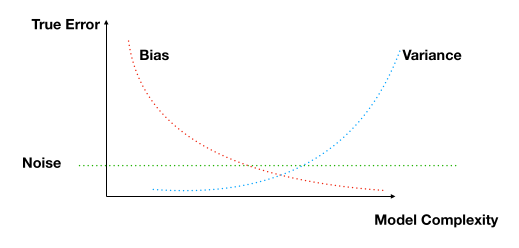
\includegraphics[width=.9\linewidth]{figures/bias-variance-tradeoff.png}
	\caption{Bias-Variance Trade-off}
	\label{fig:bias-variance-tradeoff}
    \end{subfigure}%
    \begin{subfigure}{.5\textwidth}
	\centering
	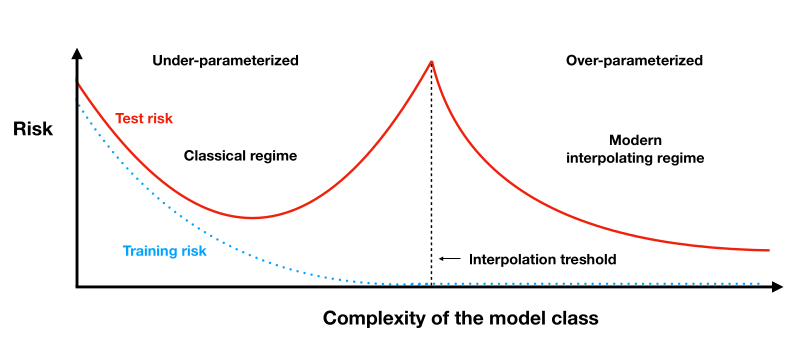
\includegraphics[width=.9\linewidth]{figures/double-descent-curve.png}
	\caption{Double Descent Curve}
	\label{fig:double-descent-curve}
    \end{subfigure}
\end{figure}


\subsection{Model Selection and Validation}

As we'll see with more detail in the following sections, there are a variety of Machine Learning models that are with different architectures, training algorithms, and tuned by different parameters.
It is thus a very relevant question how to select the best of these models.

In order to answer this question, we frame a probabilistic setup for learning.
In this setup we assume our training data $S$ is a set of observations $s$ drawn from an unknown distribution $\dist$.
As we already saw, we use a training algorithm $\mathcal{A}$ to find a prediction function $\mathcal{A}(S, \eta) = f_{S, \eta}$.
We call the \textbf{true / expected risk / error / loss} of the function $f$ to the value
$$
\loss_\dist(f) = \E_{s \sim \dist} \left[ \loss(s \mid f) \right]
$$
The fundamental issue with evaluating this loss is, however, that the distribution $\dist$ is unknown.

To cope with this limitation, we use the \textbf{empirical risk / error / loss}
$$
\loss_S(f) = \frac{1}{|S|} \sum_{s \in S} \loss(s \mid f)
$$
By linearity of expectation we have that $\E_{s \sim \dist}\left[\loss_S(s \mid f)\right] = \loss_\dist(f)$ and, thus, by Law of Large Numbers, $\loss_S(f) \to_{|S| \to \infty} \loss_\dist(f)$ but there are fluctuations.
We give the name of \textbf{generalization gap} to the quantity $|\loss_\dist(f) - \loss_S(f)|$.

Note however, that when we use the same dataset $S$ for the training algorithm and loss computation, we might overfit and $\loss_S(f_{S, \eta})$ might not converge to $\loss_\dist(f_{S, \eta})$.
Therefore, it is usual in order to evaluate the quality of a model to \textbf{split} the available data into \textbf{training data} $S_{\text{train}}$ and \textbf{testing data} $S_{\text{test}}$.
Then, we learn the prediction function $f$ on the training set through $\mathcal{A}(S_{\text{test}}, \eta)$ and validate it on the test set computing $\loss_{S_{\text{test}}}(f)$.
Now, since $S_{\text{test}}$ and $S_{\text{train}}$ are independent, $\loss_{S_{\text{test}}}(f) \approx \loss_\dist(f)$.
This strategy of splitting data of course has the disadvantage of leaving less data for both the learning and validation tasks.

Due to Hoeffding inequalities, if we can bound the loss function $\loss(s \mid f)$ in a range $[a, b]$, then for $S_{\text{test}} \sim \dist$:
$$
\prob \left[
    | \loss_\dist(f) - \loss_{S_{\text{test}}}(f) | \geq
    \sqrt{\frac{(b-a)^2 \ln(2/\delta)}{2|S_{\text{test}}|}}
\right] \leq \delta
$$
which gives us a high probability bound (the size of the bounding interval only increases logarithmically with the probability upper bound $\delta$) that also decreases proportionally with $\sqrt{|S_{\text{test}}|}$.
This bound allows us to obtain a probabilistic upper bound on the expected risk.

\paragraph{Hyperparameter Tuning}

Let's say we have a training algorithm $\mathcal{A}(S, \eta)$ for some training parameters $\eta \in \mathcal{H}$.
We can use techniques similar to the ones describes above to determine the best value of $\eta$ for training - i.e, we devise a training algorithm that solves the problem
$$
\min_{\eta \in \mathcal{H}} \loss_{S_{\text{test}}} (s \mid \mathcal{A}(S_{\text{train}}, \eta))
$$

By a simple union bound, the loss of this model is still not too far from the true loss (the generalization error increases only to $\sqrt{\frac{(b-a)^2 \ln(2K/\delta)}{2|S_{\text{test}}|}}$ where $K$ is the cardinality of $\mathcal{H}$).

\paragraph{K-fold Cross-Validation}

An alternative to splitting the data into training and test data and thus losing data for both tasks is to randomly partition the data into $K$ groups and train $K$ times, each time leaving out exactly one of the $K$ groups for testing and using the remaining $K-1$ for training.
We can then average the $K$ results for a measure of the accuracy of the model.

\paragraph{Evaluation Set}

Note that, in some tasks, when we select hyperparameters as
$$
\eta^\star = \min_{\eta \in \mathcal{H}} \loss_{S_{\text{test}}} (s \mid \mathcal{A}(S_{\text{train}}, \eta))
$$
we are to some degree using the test set in our training.
As such, a third separate \textbf{evaluation set} may be used to measure the quality of the model.

\section{Supervised Learning}

We call \textbf{Supervised Learning} to instances of learning where we are given a dataset $(X, Y) \in (\mathcal{X} \times \mathcal{Y}) \times N$ where $\mathcal{X}$ and $\mathcal{Y}$ are, respectively, the sets of possible inputs and outputs, and each pair $(x, y)$ is an observation or an instance of our dataset. 
The set $\mathcal{X}$ can be decomposed in $\mathcal{X} = \bigtimes_{i=1}^D \mathcal{F}_i$ where each $\mathcal{F}_i$ is a set of possible values of a certain \textbf{feature}.
We will usually consider $\mathcal{X} \subset \R^D$ and $\mathcal{Y} \subset \R$.
We say $D$ is the \textbf{dimensionality} of the input and $N$ is the \textbf{size} of the dataset.

The purpose of supervised learning is to learn some mapping that fits the provided dataset best. 
That is, for some loss or error function $\loss$, we shall learn a mapping $\hat{f}$ such that $\loss(\hat{f}(X), Y)$ is minimized.

\subsection{Regression}

In regression tasks we are interested in describing relations between input and output variables, whether in order to make predictions or simply understand the effect of the input on the output.

\subsubsection{Linear Regression}

For \textbf{Linear Regression} we assume that the outputs are a linear function of the inputs, and thus our function $\hat{f}$ can be written as $\hat{f}(x) = w^T \tilde{x}$ for some $w \in \R^{D+1}$.
We define $\tilde{x} = (1, x)$ and $w$ to have $D+1$ columns so that our functions can have a bias term.

Therefore, we want to find $w^\star = \arg \min_w \loss(\tilde{X}w, Y)$, and our predictions will be of the form $\hat{f}(x) = {w^\star}^T \tilde{x}$.

The most standard way to define $\loss$ is to use the \textbf{Mean Squared Error} (MSE).
This is one of rare cases where computing an optimum of the cost function analytically is possible.
The set of linear equations $\nabla \loss(w^\star) = 0$ that outputs this solution are called \textbf{normal equations} and, in the case of linear regression with MSE are:
$$
\tilde{X}^T (y - \tilde{X}w) = 0
$$
and yield
$$
w^\star = (\tilde{X}^T \tilde{X})^{-1} \tilde{X}^T Y
$$

This is called the \textbf{Least Squares} solution of linear regression with MSE.

The Euclidean norm arises naturally by assuming that the errors are normally distributed.
In fact, if we assume that the random variable $\tilde{X}w - Y$ is normally distributed with mean zero and variance $\sigma^2$, then the \textbf{Maximum Likelihood Estimation} for $w$ is the one that minimizes the MSE.

Note that $\tilde{X}^T \tilde{X}$, called the \textbf{Gram matrix}, is a symmetric matrix, and is invertible if and only if it has full column rank.
This means that we can only use this method if $D < N$.
Even if this is the case, the matrix $X$ can be \textbf{rank deficient} if some of the columns are (nearly) collinear.
When the matrix is rank deficient, we can still solve least squares using a linear solver.

This approach to linear regression has a complexity of $O(ND^2 + D^3)$ to compute $w^\star$, but predicts new values in $O(D)$ time.

Linear regression is very advantageous due to its simplicity and ease of interpretation.
However, it relies on a very strong assumption on how the outputs relate to the inputs.
Another advantage of linear regression is that it is easy to generalize to non-linear models to circumvent this.

\subsubsection{Nonlinear Regression}

Assume our dataset does not fit well to any linear function of the inputs. 
One way to deal with this is to use a nonlinear function of the inputs.
We can think of this as transforming our inputs in $\R^D$ to $\R^K$ through a function $\phi: \R^D \to \R^K$ and then using linear regression on the new inputs.
This allows us to fit our data to any function in the span of $\phi$.

In this case, $w^\star$ is given by
$$
w^\star = (\Phi(X)^T \Phi(X))^{-1} \Phi(X)^T y
$$
where $\Phi(X)$ is the matrix with the $\phi(x_i)$ as rows.
Just like before, we predict according to the function $\hat{f}(x) = {w^\star}^T \phi(x)$.

It is worth noting that our default assumption that $x_0 = 1$ for every vector can be viewed as a particular case of a mapping - $\phi(x) = (1, x)$.

This approach has the problem that it might not be obvious what kind of function our dataset follows.

It computes $w^\star$ in $O(f(D,N,K) + NK^2 + K^3)$ time (where $f(D,N,K)$ is the time needed to compute $\Phi$), predicting in $O(K)$ time.

\subsubsection{Locally Weighted Linear Regression}

If the outputs are a continuous function of the inputs, we can always fit a linear function locally to the data at any given point.
We can achieve this by using a weighted linear regression, where the weights are given by a function $\rho: \R^m \to \R$ that is high for points close to the point we are predicting and low for points far away.
The most commonly used function to assign weights is therefore $\rho(x) = \exp(-\frac{||x - x_i||^2}{2\tau^2})$ for some $\tau > 0$ ($x_i$ is the point we want to predict).
Therefore, in locally weighted regression, instead of minimizing $||X w - Y||^2$, we minimize $||P^{\frac{1}{2}}(X w - Y)||^2$ where $P$ is a diagonal matrix with the weights on the diagonal.
A prediction in this case is given by
$$
\hat{f}(x) = {w^\star}^T x = ((X^T P X)^{-1} X^T P^{\frac{1}{2}} Y)^T x
$$

This approach, while working almost always, is very slow, since it needs to compute the weights for every point in the dataset.
It takes the same $O(ND^2 + D^3)$ time to compute $w$ as the above methods, but needs to compute a different $w$ for every prediction.

\subsubsection{Regularization for Linear Regression}

\paragraph{Ridge Regression}

The most frequently used regularizer is the standard Euclidean norm ($L_2$-norm), that is
$$
\Omega(w) = \lambda ||w||_2^2
$$
We thus obtain the solution for the problem
$$
\min_w \frac{1}{2N}||y - Xw||_2^2 + \lambda ||w||_2^2
$$
that has solution
$$
w^\star = (X^T X + \lambda' I)^{-1} X^T y \quad (\lambda' = 2N\lambda)
$$

Using Ridge Regression also has the advantage of fixing ill-conditioning as the eigenvalues of the matrix $(X^T X + \lambda' I)$ are all at least $\lambda'$ and so it always as inverse.

\paragraph{Lasso Regression}

As an alternative measure of the complexity of the model, we can use a different norm.
A very important case is the $L_1$-norm, leading to $L_1$-regularization.
In combination with the MSE cost function, this is known as the Lasso model:
$$
\min_w \frac{1}{2N} ||y - X w||_2^2 + \lambda ||w||_1
$$

The Lasso model has the advantage of promoting sparsity in the model parameters (giving more importance to more relevant features).

\subsection{Classification}

A \textbf{classification} problem asks us to predict a value in a discrete set $\mathcal{Y}$ given an observation $x \in \mathcal{X}$.
Binary classification, as the name suggests, is a classification task where $|\mathcal{Y}| = 2$.
For these tasks, it is usual to use $\mathcal{Y} = \{0,1\}$ or $\mathcal{Y} = \{-1,1\}$

Instead of finding an hyperplane that best fits a real-valued output, a classifier finds a hyperplane that best separates (possibly in a higher dimensional space) observations from different classes.

We could use the techniques from regression on this problem.
However, this has some problems:
\begin{itemize}
    \item The predicted values are not probabilities (not in $[0,1]$);
    \item It is very sensitive to unbalanced data and extreme values;
\end{itemize}

For a binary classification task, the most sensible loss is $l(y, y') = \ind[y \neq y']$ and thus the true risk is given by
$$
\loss_\dist(f) = 
\E_\dist[\ind[Y \neq f(X)] = 
\prob_\dist[Y \neq f(X)]
$$

To the classifier that simply minimizes the true loss, we call \textbf{Bayes classifier}.
I.e, the Bayes classifier is the function
$$
f^\star(x) = \arg \max_{y \in \mathcal{Y}} \prob(Y = y \mid X = x)
$$
The Bayes classifier cannot be directly attained given that the distribution $\dist$ from where the dataset is taken is not know.

Classification models can mainly be divided in two classes:
\begin{itemize}
    \item \textbf{Parametric} models attempt to approximate $\dist$ via training data by minimizing the empirical risk on training data;
    \item \textbf{Non-parametric} models approximate the conditional distribution $\prob(Y = y \mid X = x)$.
\end{itemize}

\paragraph{Classification by empirical risk minimization}

The task of classification by empirical risk minimization as
$$
\min_{f : \mathcal{X} \to \mathcal{Y}} \loss_{\text{train}}(f) =
\frac{1}{N} \sum_{(x, y) \sim S_{\text{train}}} \ind[f(x) \neq y]
$$
has the problem of not being convex: $\mathcal{Y}$ is discrete and thus not convex, as is the indicator function $\ind$ since it is not continuous.

We circumvent this problem by considering convex relaxations of the classification risk.
Instead of learning $f : \mathcal{X} \to \mathcal{Y}$, we learn $g : \mathcal{X} \to \R$ in a convex subset and predict with $f(x) = \text{sign}(g(x))$.
We further use a convex surrogate $\phi : \R \to \R$ of the indicator function, obtaining the problem
$$
\min_{g \in \mathcal{G}} \frac{1}{N} \sum_{(x, y) \sim S_{\text{train}}} \phi(g(x) y)
$$
which is convex.

Furthermore, under certain technical assumptions on the function $\phi$ it is possible to bound the true error $\loss(f)$ on convex relaxation risk.

\subsubsection{Logistic Regression}

If we define $h_w(x) = \prob[y = 1 \mid x ; w]$, then we can write for $\mathcal{Y} = \{0,1\}$
$$
\prob[ y \mid x ; w ] = h_w(x)^y (1 - h_w(x))^{1 - y}
$$
Therefore, if do a MLE for $w$, we find that 
\begin{gather*}
w^\star =
\arg \max_w \prod_{(x,y) \in D} \prob(x, y \mid w) =
\arg \max_w \prod_{(x,y) \in D} h_w(x)^y (1 - h_w(x))^{1 - y} =
\arg \min_w \loss(w)
\end{gather*}
where 
$$
\loss(w) = \frac{1}{N} \sum_{(x,y) \in D} y \log(h_w(x)) + (1-y) \log(1-h_w(x))
$$
The function that is usually used for $h_w(x)$ is the sigmoid function over a linear combination of the inputs:
$$
h_w = \sigma(w^T x)
$$
where $\sigma(z) = \frac{1}{1 + \exp(-z)}$.
This choice can be explained by the Theory of Generalized Linear Models, which we will touch bellow.
The sigmoid function has a few convenient properties:
\begin{itemize}
    \item $\sigma(z) \in [0,1]$ which allows interpretation has probability;
    \item $\sigma'(z) = \sigma(z)(1-\sigma(z))$ which helps in computation of methods like gradient descent;
\end{itemize}

With this choice, our problem becomes
$$
w^\star = 
\arg \min_w \loss(w) =
\arg \min_w \frac{1}{N} \sum_{(x,y) \in D} -y x^T w + \log(1 + e^{x^T w})
$$
which is a convex problem: the loss is convex and $w$ is on a convex set.
Therefore, we can use standard convex optimization techniques on the problem.
The gradient of the loss to be used in gradient descent is 
$$
\nabla \loss(w) = \frac{1}{N} X^T (\sigma(Xw) - y)
$$

This method solves most of the problems that arose when just using regression techniques on classification.
With this setup, we can interpret the learned parameter $w^\star$ as follows:
\begin{itemize}
    \item As the decision boundary is $\sigma(w^{\star T} x) = 1/2 \Leftrightarrow w^{\star T} x = 0 \Leftrightarrow w^\star \perp x$, the weight vector is orthogonal to the decision boundary;
    \item The magnitude of the vector $||w^\star||$ is indicative of how fast the transition is from negative to positive predictions;
    \item The bias term on $w^\star_0$ informs how far on the vector the transition happens.
\end{itemize}

\paragraph{Problem when the data is linearly separable}

Note that when the data is linearly separable, increasing the magnitude of the weight vector always minimizes the loss.
Therefore, in order to prevent infinite training, one can add $L_2$ regularization to prevent the size of $w$ to increase too much.

\subsubsection{Support Vector Machines}

The idea behind Support Vector Machines is that the best separator between two linearly separable classes is the one that maximizes the \textbf{margin} between them.

The margin of a hyperplane $H$ in relation to some dataset $D$ is defined as the quantity
$$
\min_{p \in H, x \in D} ||p-x|| = \min_{x \in D} |w^T x|
$$
if $H = \{ x : w^T x = 0 \}$.

\paragraph{Hard SVM Rule}

The max-margin separating hyperplane is thus given by some vector $w^\star$ given by
$$
\max_{w, ||w||=1} \min_{x \in D} |w^T x| \quad \text{s.t } y x^T w \geq 0 \ \forall x, y \in D
$$
where we restrict $||w||=1$ so that all vectors correspond to different hyperplanes.
This formulation can be rephrased as
\begin{gather*}
\max_{M \in \R, w, ||w||=1} M \quad \text{s.t. } y x^T w \geq M \ \forall x, y \in D 
\quad \quad \text{ or } \quad \quad
\min_w \frac{1}{2}||w||^2 \quad \text{s.t. } y x^T w \geq 1 \ \forall x, y \in D
\end{gather*}

\paragraph{Soft SVM}

This technique can be extended to not linearly separable training sets by allowing positive slack variables $\xi_i, \cdots, \xi_N$ and rephrasing the problem as
$$
\min_{w, \xi} \frac{\lambda}{2} ||w||^2 + \frac{1}{N} \sum_{n=1}^N \xi_n
\quad \text{such that } y_n x_n^T w \geq 1 - \xi \text{ and } \xi_n \geq 0 \ \forall n \in \{1, \cdots, N\}
$$
which is equivalent to
$$
\min_w \frac{\lambda}{2} ||w||^2 + \frac{1}{N} \sum_{(x,y) \in D} [1 - y x^T w]_+
$$

where $[z]_+ = \max\{0, z\}$ is the Hinge loss.

As this problem is convex but non-smooth, we can minimize it with subgradient methods.

Note that the problem is in the aforementioned Empirical Risk Minimization form with $g(x) = w^T x$, $\phi$ the Hinge loss (which is a convex surrogate of the 0-1 loss) and a $L_2$ regularization term.

Using convex duality, this problem can be further rephrased as
\begin{gather*}
\max_{\alpha \in [0,1]^n} \min_w \frac{1}{N} \sum_{n=1}^N 
    \alpha_n (1 - y_n x_n^T w) + \frac{\lambda}{2} ||w||_2^2 = \\
\max_{\alpha \in [0,1]^n} 
\frac{\mathbf{1}^T \alpha}{N} - \frac{1}{2\lambda N^2} \alpha^T \mathbf{Y}XX^T\mathbf{Y}^T \alpha \quad \text{where } \mathbf{Y} = \text{diag}(Y)
\end{gather*}

where, for $G(w, \alpha) = \alpha_n (1 - y_n x_n^T w) + \frac{\lambda}{2} ||w||_2^2$ we took advantage of the fact that $\nabla_w G(w, \alpha) = 0 \Leftrightarrow w = \frac{1}{\lambda N} X^T \mathbf{Y} \alpha$. 

This interpretation has the following advantages:
\begin{itemize}
    \item It is a \textbf{differentiable concave problem} which can be efficiently solved using methods such as quadratic programming solvers and coordinate ascent;
    \item \textbf{Kernel Matrix Dependency}: The cost function only depends on the data via the \textbf{kernel matrix} $K = XX^T \in \R^{N \times N}$ - no dependency on the size of the feature space $D$;
    \item \textbf{Dual Formulation Insight}: $\alpha$ is typically sparse and non-zero exclusively for the training examples that are crucial in determining the decision boundary.
    Namely, one can observe that $\alpha_n > 0$ only if the corresponding observation is not on the correct side or if it is inside the margin.
    These are called the \textbf{support vectors} of the classifier.
    Further, as $w = \frac{1}{\lambda N} \sum_{n=1}^N \alpha_n y_n x_n$, we can conclude that $w$ depends only on the observation that are inside the margin or misclassified.
\end{itemize}

\subsection{Kernel Trick}

The Kernel trick bases itself on the observation that the \textbf{kernel matrix} $K = X X^T$ has dimensions $N \times N$.
Thus if we can make a problem depend on the dataset only through this matrix, the size of the computation will only depend on the number of datapoints, and not the size of the feature space.
This allows us to embed the problem in larger feature spaces through a feature map $\phi : \R^N \to \R^K$ obtaining a new kernel matrix $K = \Phi \Phi^T$ with entries $K_{i,j} = \phi(x_i)^T \phi(x_j)$.

However, computing the dot product $\phi(x_i)^T \phi(x_j)$ is $O(K)$ and thus too costly for $K >>$.
The kernel trick is thus to find a \textbf{kernel function} $\kappa : (\R^d)^2 \to \R$ such that $\kappa(x_i, x_j) = \phi(x_i)^T \phi(x_j)$ and that can be computed more efficiently.

However, if we want to make linear predictions on $\phi(x)$, we still have to compute $\phi(x)^T w^\star$ in $O(K)$ time.
This is where the \textbf{Representer Theorem} comes in:

\paragraph{Representer Theorem}:
For any loss function $l$ there exists $\alpha^* \in \R^N$ such that
$$
w^* = X^T \alpha^* \in \arg \min_w \frac{1}{N} \sum_{n=1}^N l(x_n^T w, y_n) + \frac{\lambda}{2} ||w||^2
$$

From this, we can conclude there is always an optimal solution within $\text{span} \{ x_1, \cdots, x_N \}$ for a linear regression problem with $L_2$ regularization and any loss function.

Thus, when we expand the feature space, we can write $w^\star$ as $\Phi^T \alpha^\star$ for some $\alpha^\star \in \R^N$ and we can rewrite $\phi(x)^T w^\star = \phi(x)^T \Phi^T \alpha^\star = \sum_{n=1}^N \kappa(x, x_n) \alpha^\star_n$ which we can compute in $O(NT)$ where $O(T)$ is the computation time for the kernel function.

\paragraph{Kernel Ridge Regression}

$$
\min_w \frac{1}{2N} \sum_{n=1}^N (y_n - w^T x_n)^2 + \frac{\lambda}{2}||w||^2 = 
\frac{1}{N} X^T \left( \frac{1}{N} X X^T + \lambda I_N \right)^{-1} y
$$
I.e
$$
w_* = X^T \alpha_* \text{ where } \alpha_* = \frac{1}{N} \left( \frac{1}{N} X X^T + \lambda I_N \right)^{-1} y \quad \Rightarrow \quad
w_* \in \text{span}\{x_1, \cdots, x_N\}
$$
where $\alpha_*$ can be given by the alternative formulation
$$
\alpha_* = \arg \min_\alpha \frac{1}{2} \alpha^T \left( \frac{1}{N} XX^T + \lambda I_N \right)^{-1} \alpha - \frac{1}{N} \alpha^T y
$$

\paragraph{Examples of Kernels}

\begin{itemize}
    \item \href{https://en.wikipedia.org/wiki/Polynomial_kernel}{\textbf{Polynomial Kernel}}: $\kappa(x, x') = (x^T x' + c)^d$
    \item \href{https://en.wikipedia.org/wiki/Radial_basis_function_kernel}{\textbf{Radial Basis Function (RBF) kernel}}: $\kappa(x, x') = e^{-(x-x')^2}$\\
	is a kernel of particular interest because the feature vector 
	$\phi(x) = e^{-x^2} \left( \cdots, \frac{2^{k/2} x^k}{\sqrt{k!}}, \cdots \right)$
	is infinite-dimensional.
\end{itemize}

\paragraph{Building new kernels from existing kernels}

If $\kappa_1, \kappa_2$ are two kernels then:
\begin{itemize}
    \item $\kappa(x, x') = \alpha \kappa_1(x, x') + \beta \kappa_2(x, x')$
	is a kernel for all $\alpha, \beta \geq 0$
    \item $\kappa(x, x') = \kappa_1(x, x') \kappa_2(x, x')$
	is a kernel
\end{itemize}

\paragraph{Mercer's condition}

Given a function $\kappa$, there is a map $\phi$ such that $\kappa(x, x') = \phi(x)^T \phi(x')$ if and only if
\begin{itemize}
    \item The function is symmetric: 
	$\forall x, x', \kappa(x, x') = \kappa(x', x)$
    \item The kernel matrix is PSD for all possible input sets:
	$\forall S = \{x_1, \cdots, x_L \}, \ K = (\kappa(x_i, x_j))_{i,j=1}^L \succeq 0$
\end{itemize}

\subsection{k Nearest Neighbours}

The \textbf{k Nearest Neighbours} algorithm is a very simple algorithm that can be used for both regression and classification and simply considers the outputs of the $k$ nearest datapoints to determine the prediction for a new datapoint.
This of course implies that a metric must be defined to measure distances between points, with common choices being the Euclidean ($L_2$), Manhattan ($L_1$), Minkowski ($L_p$), Cosine ($1 - \frac{x \cdot y}{||x|| ||y||}$) and Hamming ($\sum_{i=1}^k \ind[ x_i \neq y_i ]$) (for categorical features) distances.

It is important to note that the different features might be on very different scales, thus attributing very different relevance to the distances in those axis.
Therefore it is usually important to \textbf{normalize} the vectors before computing the distances.

The kNN predictor therefore works by just gathering the $k$ nearest neighbours and computing an estimator for the output using the neighbours.
Frequent estimators are the mean or median for regression problems and majority vote or weighted majority for classification problems.

On must carefully choose the value of $k$ when using kNN: a small value will lead to decision boundaries that are too complex and too adjusted to noise in the data - overfitting.
On the other side, large values of $k$ will lead to too inflexible models with a high bias - underfitting.

kNN has the advantage of needing no optimization or training, being simple to understand and easy to implement and works well in low dimensions with data that has significant spacial correlation.
However, it is slow at query time, not suitable for high-dimensional data due to the curse of dimensionality and choosing the right local distance is crucial.

\subsection{Generalized Linear Models}

%TODO
This is not on the exam... Maybe someday I'll have the time to fill this in.

\subsection{Naive Bayes}

We can use \textbf{Bayes Theorem} to find the most probable hypothesis $\hat{H}$ given some data $D$.
\begin{gather*}
\hat{H} = \arg \max_{H} P(H \mid D) = \arg \max_{H} \frac{P(D \mid H)P(H)}{P(D)} = \arg \max_{H} P(D \mid H)P(H) = \\
= \arg \max_{H} \prod_{d \in D} P(d \mid H)P(H) = \arg \max_{H} \prod_{d \in D} P(d_1, \cdots, d_k \mid H)P(H)
\end{gather*}
We say that $\hat{H}$ is the \textbf{Maximum A Posteriori} (MAP) hypothesis, i.e, it is the most likely hypothesis after we observe the data.

If the data is multifeatured, evaluating $P(d \mid H)$ for some observation $d$ might be complicated.
If we are only given information about each feature $d_i$ individually, we can only compute their probabilities independently.
However, in general, the features have some correlation, causing this calculation to be tougher.

On a \textbf{Naive Bayes} classifier we assume that the features are independent, thus simplifying significantly the calculations.
In this case, for an observation $d$, we have
\begin{gather*}
P(d \mid H) = \prod_{i=1}^k P(d_i \mid H)
\end{gather*}
and we can get the probabilities inside the product by referring to the distribution of each feature.

Note that this assumption is very often a bad assumption.
However, it has been observed that Naive Bayes performs well in practice, even when the features are not independent.

\subsection{Decision Trees}

Some classification problems are best modeled by a complex combination of predicates.
\textbf{Decision Trees} work well in cases where differentiating the classes can be done (or approximated well enough) by asking a series of questions.

A \textbf{Decision Tree} is a tree where each node splits the domain into sections according to a certain predicate on one of the features.
At every leave, we end up with a subset of the domain, and we can assign a class to that subset.
This is done by just taking the mode of the classes in that subset.

The obvious question that poses itself is how to select the feature at each node, and which predicate to evaluate to create the children of the current node.

We start by defining how to choose the predicate.
Normally, the predicate used is just a threshold on the value of some feature, which can be viewed as slicing the domain space at the current node in two, through an hyperplane orthogonal to the axis of the current feature.
To choose where this slice should be done, we need to define a cost function that measures how good a split is.

\section{Neural Networks}

In the methods we've seen so far we are predicting according to a function $f(x) = \phi(x)^T w$ which is a linear combination of handcrafted features that require significant expertise to uncover.

Neural Networks change the approach to learning the relevant features directly from the data.
I.e, Neural Networks will make predictions of the form $f(x) = h(x)^T w$ where the features $h(x)$ are the features extracted by the network.

\subsection{Perceptron}

The \textbf{perceptron} algorithm is a very simple algorithm for binary classification with many similarities with logistic regression, with the only change being the \textbf{activation function}, which becomes the sign function instead of the sigmoid.
Therefore, predictions are made with $\text{sign}(w^T x)$ for a parameter $w \in \R^n$ which is found by successive applications of the \textbf{perceptron update rule}:
$$
w^{(t+1)} = w^{(t)} + \gamma (y - \hat{y}) x
$$
on successive datapoints $(x,y) \in D$ where $\hat{y} = \text{sign}(w^T x)$.

The algorithm is guaranteed to converge to a solution if the data is linearly separable and $\gamma$ is sufficiently small.

It is worth noting that since the derivative of the sign function is 0 at every point (except 0, where it is not defined), we cannot use gradient descent to "teach" a perceptron, creating the need for a specific learning algorithm.

\subsection{Fully Connected Neural Networks}

Multi-layer Neural Networks emerge from the idea that if we combine several perceptron-like structures - which we'll refer to as \textbf{nodes} or \textbf{neurons} - we are able to learn much more complicated patterns than those we can learn with a single one.
Therefore, these architectures are made of:
\begin{itemize}
    \item An \textbf{input layer} where the features $x_1, \cdots, x_D$ are provided;
    \item Several \textbf{hidden layers} where the features in a previous layer are linearly combined and then subject to some application function.
	I.e, let $x^l_i$ be the $i$-th node of the $l$-th layer of the net. Then
	$x^l_i = \phi^l_i({w^l_i}^T x^l_i + b^l_i)$
	where $\phi^l_i$ is the node's activation function and $w^l$ and $b^l$, respectively, the weights and biases on the $l$-th layer.
    \item An \textbf{output layer} that works similarly as the hidden layers.
\end{itemize}

Note that each node may have its own activation function. 
However, it is usual that all nodes use the same activation function, except possibly for those in the output layer, whose activation function will depend on the kind of task we want to perform.
Furthermore, we will start our discussion only with Neural Networks that have $L+1$ layers and $K$ nodes per hidden layer.

For these types of structures, a Neural Network is then formalized with:
\begin{itemize}
    \item $L+1$ variables $x^0, \cdots, x^L$ with $x^0 \in \R^D$, $x^i \in \R^K$ for $i \in \{1, \cdots, L-1\}$ and $x^L \in \R^O$ where $\R^O$ is the output space of our problem;
    \item An activation function $\phi : \R \to \R$ and a prediction function $p : \R \to \R$ (which will arbitrarily be used element wise over vectors).
	Usual choices for the activation function are traditionally the sign and the sigmoid functions and, nowadays, the ReLU $\phi(x) = (x)_+ = \max\{0,x\}$ and the GeLU $\phi(x) = x \Phi(x) \approx x \sigma(1.702x)$ are more widely used.
	The prediction function depends on the task we want to perform
	\begin{itemize}
	    \item For regression tasks, it is usual to just predict with the linear combination of the last hidden layer: 
		$p(x) = x$ 
		with a squared loss 
		$l(y, h(x)) = (h(x) - y)^2$;
	    \item For binary classification tasks with $\mathcal{Y} = \{-1, 1\}$ it is usual to use the sign function 
		$p(x) = \text{sign}(x)$
		with the cross-entropy loss
		$l(y, h(x)) = \log(1 + \exp(-yh(x)))$;
	    \item For multiclass classification it is usual to use 
		$p(x) = \arg \max_{c \in \mathcal{Y}} h(x)_c$
		with the softmax loss
		$l(y, h(x)) = -\log \frac{\exp(h(x)_y)}{\sum_{c \in \mathcal{C}} \exp(h(x)_c)}$.
	\end{itemize}
    \item Weight matrices $W^1, \cdots, W^L$ with $W^1 \in \R^{K \times D}$, $W^i \in \R^{K \times K}$ for $i \in \{2, \cdots, L-1\}$, and $W^L \in \R^{O \times K}$;
    \item Bias vectors $b^1, \cdots, b^L$ with $b^i \in \R^K$ for $i \in \{1, \cdots, L-1\}$ and $b^L \in \R^O$.
\end{itemize}

With these definitions in hand, we can express each layer with $x^l = \phi(W^l x^{l-1} + b^l)$ for each hidden layer and $x^L = p(W^L x^{L-1} + b^L)$.
In order to ease notation, it usual to let $z^l = W^l x^{l-1} + b^l$, so that $x^l = \phi(z^l)$.

We note that all the weight matrices and bias vectors parametrize the neural network.
These are the values that we want to learn from the data.
We can see that the number of parameters is $(DK + K^2(L-2) + KO) + (K(L-1) + O) = O(K(D + KL + O)) = O(K^2L)$ in most cases.
In practice, $L$ and $K$ are usually large making the Neural Networks overparametrized.

The prediction process of a neural network given an input $x$, called \textbf{Forward Propagation} is then as follows:
\begin{enumerate}
    \item Set $x^1 = x$.
    \item For $l = 2, \dots, L$:
    \begin{enumerate}
	\item Compute $z^l = W^l x^{l-1} + b^l$.
	\item Compute $x^l = f(z^l)$.
    \end{enumerate}
    \item Return $\hat{y} = x^L$.
\end{enumerate}

\subsubsection{Representational Power of NNs}

\paragraph{Barron's Result}

Let $f : \R^d \to \R$ and $\hat{f}(\omega) = \int_{\R^d} f(x) e^{-i\omega^Tx} \ dx$ be its Fourier transform.
If $\int_{\R^d} |\omega| |\hat{f}(\omega)| \ d \omega \leq C$ (smoothness assumption) then $\forall n \in \Z^+, r \in \R^+$, there exists a function $f_n$ of the form
$$
f_n(x) = \sum_{j=1}^n c_j \phi(x^T w_j + b_j) + c_0
$$
for some $w_1, \cdots, w_n \in \R^d$, $b_1, \cdots, b_n \in \R$, $c_0, \cdots, c_n \in \R$ such that
$$
\int_{|x| \leq r} (f(x) - f_n(x))^2 \ dx \leq \frac{(2Cr)^2}{n}
$$

Note that for Barron's Result, the approximation is on average (in $L_2$ norm).
It concludes that any "sufficiently smooth" function can be approximated by a one-layer NN (with a sigmoid-like activation function)·

\paragraph{$L_1$ Approximation}

Let $f$ be a Riemann-integrable function on $[a,b]$.
By definition, for any $\epsilon > 0$ there are $n >> , a = i_0, i_1, \cdots, i_{n-1}, i_n = b$, such that the function $f_n(x) = \inf_{x \in [i_k, i_{k+1}]} f(x)$ if $x \in [i_k, i_{k+1}]$ satisfies
$$
\int_a^b |f(x) - f_n(x)| dx < \epsilon
$$

$f_n$ is what is called a rectangle function.
Observing that any rectangle function (in any dimension) can be approximated by a sigmoid of a linear combination of sigmoids of linear combinations, we can conclude that any sigmoid-activated one-layer NN can approximate any Riemann-integrable function.

\paragraph{Point-Wise Approximation}

Let $f$ be a continuous function on $[a,b]$.
For all $\epsilon > 0$, it exists a piecewise linear function $q$ such that
$$
\sup_{x \in [a, b]} |f(x) - q(x)| \leq \epsilon
$$

One can see that any piece-wise function can be written as a linear combination of RELU functions.
As such, any ReLU-activated one-layer NN can approximate any continuous function.

\subsubsection{Backward Propagation}

The only thing remaining is then to find a way to learn these parameters.
We can do this by using the \textbf{Backpropagation} algorithm, which is essentially a form of stochastic gradient descent.

We see that for any layer
$$
\frac{\partial \loss}{\partial W^l} = 
\frac{\partial \loss}{\partial z^l} \frac{\partial z^l}{\partial W^l} =
(x^{l-1} \nabla_{z^l} \loss)^T
\quad \quad \quad
\frac{\partial \loss}{\partial b^l} = 
\frac{\partial \loss}{\partial z^l} \frac{\partial z^l}{\partial b^l} =
(\nabla_{z^l} \loss)^T
$$

Furthermore, noting that
$$
\frac{\partial \loss}{\partial z^l} =
\frac{\partial \loss}{\partial z^{l+1}} \frac{\partial z^{l+1}}{\partial x^l} \frac{\partial x^l}{\partial z^l} =
\left( \nabla_{z^{l+1}} \loss \cdot W^{l+1} \right)^T \odot \phi'(z^l)
$$

we can reuse the derivatives computed in a layer for the previous one.
Therefore, we can now describe the backpropagation algorithm as follows:
\begin{enumerate}
    \item Set $x^1 = x$.
    \item Forward propagate the input through the network, computing $z^l$ and $x^l$ for each layer.
    \item Compute $\delta^L \in \R^O$ with entries $\delta_i = \frac{\partial \loss}{\partial z^L_i} = \loss'(x^L_i) p'(z^L_i)$
    \item For $l = L-1, \dots, 1$:
    \begin{enumerate}
	\item Compute $\frac{\partial \loss}{\partial W^l} = \delta^l {x^{l-1}}^T$.
	\item Compute $\frac{\partial \loss}{\partial b^l} = \delta^l$.
	\item Update the parameters as follows:
	$$
	W^l \leftarrow W^l - \eta \frac{\partial \loss}{\partial W^l} \quad \quad \quad
	b^l \leftarrow b^l - \eta \frac{\partial \loss}{\partial b^l}
	$$
    \item Compute $\delta^{l-1} = \left( {W^{l-1}}^T \delta^l \right) \odot \phi'(z^{l-1})$ if $l \neq 1$.
    \end{enumerate}
\end{enumerate}

\subsection{General Considerations and Enhancement Strategies}

\subsubsection{Parameter Initialization}

While parameter initialization bears little significance in convex problems, the minimization of a NN is not a convex problem and in deep networks, improper parameter initialization can lead to the vanishing or exploding gradients problem, which cause either slow or unstable optimization.

A possible solution is to control the layer wise variance of the neurons.

Another possible method is introducing Normalization Layers.

\paragraph{Batch Normalization}

Consider a batch $B = (x_1, \cdots, x_M)$ of observations.
We'll normalize each layer's input using its mean and variance over the batch.
I.e, we compute $\mu_B^l$ and $(\sigma_B^l)^2$, and for $z_n^l$ the pre-activation value of layer $l$ for input $x_n$
$$
\overline{z}_n^l = \frac{z_n^l - \mu_B^l}{\sqrt{(\sigma_B^l)^2 + \epsilon}}
$$
for some $\epsilon \geq 0$ that is added for numerical stability.

We then introduce learnable parameters $\gamma^l, \beta^l \in \R^K$ to be able to reverse the normalization if needed.

In order to be able to make predictions, we compute $\hat\mu^l = \E [ \mu_B^l]$ and $\hat\sigma^l = \E[\sigma_B^l]$ during training, using them for inference.
Exponential moving averages are commonly used in practice.

This method has the disadvantage of requiring sufficiently large batches to get good estimates of $\mu_B^l$ and $\sigma_B^l$.
However, it leads to much faster convergence and allows to use much larger learning rates.

\paragraph{Layer Normalization}

For this method we normalize each layer's input using its mean and variance over the features.
I.e, for $\mu_n^l = \frac{1}{K} \sum_{k=1}^K z_{n,k}^l$ and $(\sigma_n^l)^2 = \frac{1}{K} \sum_{k=1}^K (z_{n,k}^l - \mu_n^l)^2$, and $\epsilon \geq 0$, we compute
$$
\overline{z}_n^l = \frac{z_n^l - \mu_n^l \cdot \mathbf{1}_K}{\sqrt{(\sigma_n^l)^2 + \epsilon}}
$$
and, again, introduce learnable parameters $\sigma^l, \beta^l \in \R^K$.

\subsubsection{Skip Connections}

Skip connections come from the realization that adding more layers does not, as it would be expected, necessarily maintain/decrease the training loss.

The solution is then found to be to add skip connections around some layers, thus transforming the value of a layer $Y$ from $Y = F(X)$ ($X$ the previous layer) to $Y = F(X) + X$.

\subsubsection{Data Augmentation}

Data augmentation is a technique where we come up with transformations $\tau : \R^d \to \R^d$ which preserve labels ($y_x = y_{\tau(x)}$) and expand our dataset from $S_\text{train}$ to $S_\text{train} \cup \{ (\tau(x), y) \}_{(x,y) \in S_\text{train}}$.

This strategy, which can be seen as a type of regularization, not only gives us more training data but encourages the model to be invariant to $\tau$.

\subsubsection{Weight Decay}

It is standard practice to regularize weights without regularizing bias terms:
$$
\min \loss + \frac{\lambda}{2} \sum_l ||W^l||^2_F
$$

\subsubsection{Dropout}

The dropout technique is defined by at each training step consider each node in a layer $l$ with probability $p^l$.

\subsection{Convolutional Neural Networks}

The fully connected NNs we have been looking at have many parameters and do not capture spatial dependencies.

Convolutional NNs (CNNs) tackle this problem by alternating two types of layers:
\begin{itemize}
    \item \textbf{Convolutional layers} that capture spatial relations
    \item \textbf{Pooling layers} that perform spatial downsampling
\end{itemize}

This architecture then includes a fully connected NN at the end to solve the problem based on the features extracted by the rest of the network.

A convolution is an operation that uses a filter matrix $F \in \R^{k \times l}$ to transform a matrix $X^0 \in \R^{n \times m}$ into a matrix $X^1 \in \R^{(n-k) \times (m-l)}$ following the rule
$$
X_{i,j}^1 = F \odot [X^0]_{i-k',j-l'}^{i+k',j+l'}, \text{ for } i \in \{k', \cdots, n-k'-1\}, j \in \{l', \cdots, m-l'-1\}
$$
with $k = 2k'+1, l=2l'+1$.

Note that the operation is not defined on the borders of the original matrix.
This can usually be dealt with in one of two ways:
\begin{itemize}
    \item \textbf{Zero padding}: the original matrix is padded with 0s around the border so that the operation is defined for all entries.
    \item \textbf{Valid padding} we perform the convolution only on the entries where the convolution is defined, reducing the size of the matrix.
\end{itemize}

On CNNs the learned parameters are the weights of the convolution.
For this architecture we usually use the same filter at every position - \textbf{weight sharing} - which makes the number of parameters much smaller and thus the training much faster. 
Backpropagation can run normally on these weights and we then sum the gradients of all edges that share the same weight.
For inputs with multiple channels, however, it is usual to use different filters for different channels.
The hyperparameters of the convolutional layer are the size, padding and stride of the filter.

For the pooling layers, we also must define the size, type, and stride of the pooling operation.
Some usual types of pooling operations are \textbf{max pooling} and \textbf{average pooling}.

A non-linear function $\phi$ (such as ReLU) is included after each convolutional layer to make the model non-linear).

\subsection{Transformers}

Many interesting problems in ML can be expressed as mapping one sequence to another as various types of data can be represented as sequences.

A transformer works in this sequence to sequence paradigm.
Formally, a transformer is a neural network $f: \text{sequence} \to \text{sequence}$ that iteratively transforms a sequence to another sequence and mixes the information between the sequence elements via \textbf{self-attention}.

The basic transformer architecture has 3 fundamental parts:
\begin{itemize}
    \item \textbf{Input transformation}: converts the input sequence elements into real-valued vector representations named \textbf{tokens}.
    \item \textbf{Transformer block}: transforms a sequence of $T$ vectors of dimension $D$ into a new sequence of $T$ vectors of dimension $D$.
    \item \textbf{Output transformation}: converts the vectors to the desired output format.
\end{itemize}

The transformer architecture can be used in different ways:
\begin{itemize}
    \item \textbf{Encoders} produce a fixed output size and process all inputs simultaneously.
    \item \textbf{Decoders} auto-regressively sample the next token as the most likely and use it as new input token - capable of generating responses of arbitrary length.
    \item \textbf{Encoder-decoder} first encode the whole input and then decode to token by token.
\end{itemize}

\subsubsection{Transformer Block}

The transformer block is based on \textbf{Self-Attention (SA)} that mixes information tokens and \textbf{Multi-Layer Perceptrons (MLP)} that mix information within tokens.
These blocks are usually powered with skip connections and layer normalization at the start of the residual branch as well.

\paragraph{Attention}

Attention is a function that transforms a sequence of tokens to a new sequence of tokens using a learned input-dependent weighted average.
Let there be $T_\text{in}$ input tokens in a matrix $V \in \R^{T_\text{in} \times D}$ and $T_\text{out}$ output tokens in a matrix $Z \in \R^{T_\text{out} \times D}$.
Then $Z = PV$ where $P \in [0,1]^{T_\text{out} \times T_\text{in}}$ are the weighting coefficients that form a valid probability distribution over the input tokens ($\sum_{j=1}^{T_\text{in}} p_{i,j} = 1$).

The idea behind attention is to make the weighting coefficient be based on the similarity between some \textbf{query tokens} (in this case the output tokens) and some \textbf{key tokens} (the input tokens).
$$
p_{i,j} = \frac{\exp(q_i k_j^T / \sqrt{D})}{\sum_{t=1}^{T_\text{in}} \exp \left( q_i k_t^T / \sqrt{D} \right)}
\quad \text {or, alternatively } \quad
P = \text{softmax}\left( \frac{QK^T}{\sqrt{D}} \right)
$$
Here, we use the inner product to obtain the similarity, divide by $\sqrt{D}$ to stabilize the values and the softmax to obtain a probability distribution. 

\paragraph{Self-Attention}

The idea behind self-attention is to derive the matrices $V, K, Q$ from the same input sequence $X \in \R^{T \times D}$ (note that $T = T_\text{in} = T_\text{out}$).
As such, we make $V = XW_V, K = XW_K, Q = XW_Q \in \R^{T \times D}$ with $W_V, W_K, W_Q \in \R^{D \times D}$ being learned parameters.

The output thus becomes
$$
Z = \text{softmax} \left( \frac{X W_Q W_K^T X^T}{\sqrt{D}} \right) X W_V
$$

\paragraph{Multihead Self-Attention}

It is desirable to have multiple attention patterns per layer, similar to having multiple convolutions in a convolutional layer.
Thus, it is usual to run $H$ self-attention "heads" in parallel, with the final output being obtained by concatenating the head-outputs and applying a linear transformation which is also learned through backpropagation.

\paragraph{Positional Information}

Attention by itself does not account for the order of inputs, however relevant it often is.
The solution to this is to incorporate a positional encoding in the network which is a function from the position to a feature vector $pos : \{1, \cdots , T\} \to \R^D$.
The most basic choice is to add a positional embedding $W_{pos}$ and learn it via backpropagation.

\paragraph{Mixing within Tokens}

After mixing information across tokens, transformers use Multi-Layer Perceptrons to mix information within tokens.
Each token is subject to the same transformation independently:
$$
MLP(X) = \phi(X W_1) W_2
$$
where matrices $W_1, W_2 \in \R^{D \times D}$ are learned via backpropagation.

\subsubsection{Input Transformations}

\paragraph{Text Token Embeddings}

Text tokenization is done by splitting the input text into a sequence of input tokens (typically word fragments + some special symbols) according to some predefined tokenizer procedure.
Then, the IDs of these tokens are converted to real-valued vectors through a transformation $W \cdot e_i = w_i$ where $W \in \R^{D \times N_\text{vocab}}$ is the parameter of the transformation that is learned via backpropagation.
The whole input sequence of $T$ tokens leads to an input matrix $X \in \R^{T \times D}$

\paragraph{Image Patch Embeddings}

Images are divided into patches of a given size (usually 16x16 pixels each) and flattened into a vector of size $16 \cdot 16 \cdot 3 = 768$.
These are then multiplied by an embedding matrix $W \in \R^{D \times 768}$ which is shared for all inputs.
The whole input sequence of $T$ embedded patches leads to an input matrix $X \in \R^{T \times D}$.

\subsubsection{Output Transformations}

Output transformations are typically simple: linear transformation or a small MLP.
The specifics are highly dependent on the task.

\subsection{Adversarial ML}

Neural Networks are often very unrobust in their classification.
They are very prone to \textbf{adversarial examples} where small perturbations may cause misclassification with high confidence.

In order to cope with this, one may consider, instead of the standard loss $\loss(f) = \E_\dist \left[ \ind[f(X) \neq Y]\right]$ one may take the \textbf{adversarial loss}:
$$
\loss_\epsilon(f) = 
\E_\dist \left[ \max_{\hat{X} \in B_\epsilon(X)} \ind[ f(\hat{X}) \neq Y] \right] 
$$

Like before, we'll approximate this true adversarial loss through one calculated over the training dataset and we'll use a continuous surrogate of the indicator function, leading to the robust optimization problem:
$$
\min_\theta \frac{1}{N} \sum_{(x,y) \in D} \max_{\hat{x} \in B_\epsilon(x)} l(y g_\theta(\hat{x}))
$$
where $g$ is the output of the NN pre-prediction ($f(x) = \text{sign}(g(x))$).

Note that finding $\max_{\hat{x} \in B_\epsilon(x)} l(y g(\hat{x}))$ consists in performing an attack on the neural network, i.e, finding an adversarial example to it's prediction.
We'll thus focus on this task.

\paragraph{White-box Attack}

If we know the prediction model $g$, we can compute the gradient of the loss $\nabla_x l(yg(x)) = yl'(yg(x)) \nabla_x g(x)$ and move in the opposite direction of the gradient.

Note, however, that this might move too far from $x$.
We thus may take an alternative approach which is to linearise the loss function $\tilde{l}(x) = l(yg(x))$:
$$
\max_{\hat{x} \in B_\epsilon(x)} \tilde{l}(\hat{x}) \approx
\max_{\hat{x} \in B_\epsilon(x)} \tilde{l}(x) + \nabla_x \tilde{l}(x)^T (\hat{x} - x) =
\tilde{l}(x) + \max_{||\delta|| < \epsilon} \nabla_x \tilde{l}(x)^T \delta
$$

This is a simple problem for which we can get a closed-form solution depending on the norm used to measure the perturbation size $||\delta||$:
\begin{gather*}
\hat{x} = x - \epsilon y \frac{\nabla_x g(x)}{|| \nabla_x g(x) ||_2} \quad \text{ for the } L_2 \text{ norm} \\
\hat{x} = x - \epsilon y \cdot \text{sign}( \nabla_x g(x) ) \quad \text{ for the } L_\infty \text{ norm} 
\end{gather*}

One can then do a \textbf{one-step attack}, where this step is performed just once, or a \textbf{multi-step attack}, where the step is performed several times followed by a projection on to the feasible set (i.e, the $L_2$ / $L_\infty$ balls).

The choice of the norm leads to different properties of the resulting adversarial perturbations.
For example, $L_\infty$ perturbations are dense, while those using $L_2$ are sparse.
It is left then to decide which kind of perturbations our model should be robust against.

\paragraph{Black-box Attack}

When we do not have access to the model, we can try to estimate the gradient through queries.
There are different assumptions on the knowledge about the model
\begin{itemize}
    \item \textbf{score-based}: If we can query the continuous model scores $g(x) \in \R$ we can approximate the gradient by using the finite difference formula:
	$$
	\nabla_x g(x) \approx \sum_{i=1}^d \frac{g(x+\alpha e_i) - g(x)}{\alpha}e_i
	$$
    \item \textbf{decision-based}: If we can only query the predicted class $f(x) \in \{-1, 1\}$ similar techniques can be adapted
\end{itemize}

Alternatively, we can do what's called a \textbf{transfer attack}.
We train a similar surrogate model $\hat{f} \approx f$ on similar data an transfer the resulting white-box adversarial perturbation from $\hat{f}$ to $f$.
The success of this attack depends on how similar the model architecture and data are.
If we are allowed to query $f$ given some unlabeled inputs we can use that information to learn $\hat{f}$ - known as \textbf{model stealing}.

\paragraph{Physically realizable attacks}

For practical application, adversarial examples must meet additional requirements such as resilience to JPEG compression, resilience to photographic distortions and resilience to varying camera angles.

\section{Unsupervised Learning}

We say we are in an \textbf{unsupervised learning} setting if we are given a dataset $X \in \mathcal{X}$ and we want to gather some information of any form about that data.

Two main directions in unsupervised learning are
\begin{itemize}
    \item \textbf{Representation Learning}
    \item \textbf{Density Estimation} and \textbf{Generative Models}
\end{itemize}

\subsection{Clustering}

One of the most common types of unsupervised learning is \textbf{clustering}, where we want to group together the data points in $X$ into clusters.
We define clusters as being subsets of $X$ such that the intradistances are small and the interdistances are large.

\subsubsection{K-Means}

One of the most common algorithm for clustering is \textbf{K-Means}.
In this algorithm, the objective is to find "prototype" points $\mu_1, \mu_2, \cdots, \mu_K$ and cluster assignments $z_n$ for all data vectors.
This problem is equivalent to:
\begin{gather*}
\min_{z, \mu} \loss(z, \mu) = \sum_{n=1}^N \sum_{k=1}^K z_{n,k} ||x_n - \mu_k||_2^2 \\
\text{such that } \mu \in \R^{K \times D}, z \in \{0,1\}^{N \times K}, \sum_{k=1}^K z_{n,k} = 1 
\end{gather*}

This problem can be solved with the following algorithm:
\begin{enumerate}
    \item Choose $K$ random points in $X$ as the initial prototypes $\mu_1, \cdots, \mu_k$.
    \item Repeat until convergence
    \begin{enumerate}
	\item For each point $x_n \in X$, set $z_{n,k} = \ind [k = \min_j ||x-\mu_j||^2]$.
	\item For each cluster $j$, set $\mu_j = \frac{\sum_{n=1}^N z_{n,j} x}{\sum_{n=1}^N z_{n,j}}$.
    \end{enumerate}
\end{enumerate}

This algorithm guarantees convergence to a local optimum.

K-means is a coordinate descent algorithm where, to find $\min_{z, \mu} \loss(z, \mu)$, we start with some $\mu^{(0)}$ and repeat the following, alternating:
$$
z^{(t+1)} = \arg \min_z \loss(z, \mu^{(t)}) \quad \quad \quad
\mu^{(t+1)} = \arg \min_\mu \loss(z^{(t+1)}, \mu)
$$

K-means has the problem of being computationally heavy for large $N$, $D$ and $K$, forcing the clusters to be spherical and performing hard cluster assignments.

Furthermore, it may not be clear how to select $k$.
In these situations, a common approach is to grid-search over some values.

\subsubsection{Gaussian Mixture Model and Expectation Maximization (EM)}

\paragraph{Gaussian Mixture Model}

In order to solve the issues presented by k-means, we move to the Gaussian Mixture Model (GMM) paradigm, where we assume the datapoints we receive were generated by $k$ different Gaussian distributions, and we're interested in finding their density.
On top of the prototypes $\mu_k$, we further select $K$ covariance matrices $\Sigma_k$ and define the probability of a certain point $x$ being in some cluster $k$ as
$$
p(x \mid \mu_k, \Sigma_k) = \mathcal{N}(x \mid \mu_k, \Sigma_k) = (2 \pi)^{-\frac{D}{2}} |\Sigma|^{-\frac{1}{2}} \exp \left( \frac{1}{2} (x-\mu)^T \Sigma^{-1} (x-\mu) \right)
$$
and, given some assignments $z$, we get
$$
p(X \mid \mu, \Sigma, z) = \prod_{x \in D} \prod_{k=1}^K \mathcal{N}(x \mid \mu_k, \Sigma_k)^{z_{n,k}}
$$

With this model, we solve the spherical boundaries problem, and are also in a position to solve the hard clustering problem if we make $z \in \{1, 2, \cdots, K\}$ a random variable that follows a multinomial distribution (let $\prob(z_n = k) = \pi_k$ with $\pi_k > 0$ and $\sum_{k=1}^K \pi_k = 1$)

Together, the likelihood and the prior define the joint distribution of the GMM:
$$
\prob(X, z \mid \mu, \Sigma, \pi) = 
\prod_{n=1}^N \prob(x_n \mid z_n, \mu, \Sigma) \prob(z_n \mid \pi) = 
\prod_{n=1}^N \prod_{k=1}^K \left[ \mathcal{N}(x_n \mid \mu_k, \Sigma_k) \pi_k \right]^{z_{n,k}}
$$

Here, $x_n$ are observed data vectors, $z_n$ are latent unobserved variables and the unknown parameters are given by $\theta = \{ \mu, \Sigma, \pi \}$.

GMM is a latent variable model with $z_n$ being the unobserved (latent) variables.
An advantage of treating $z_n$ as latent variables instead of parameters is that we can marginalize them out to get a cost function that does not depend on $z_n$, i.e. as if $z_n$ never existed.
Specifically, we get the following marginal likelihood by marginalizing $z_n$ out from the likelihood:
$$
p(x_n \mid \theta) = \sum_{k=1}^K \pi_k \mathcal{N}(x_n \mid \mu_k, \Sigma_k)
$$
which allows us to obtain the optimization problem
$$
\max_\theta \prob(X \mid \theta) =
\max_\theta \prod_{x \in D} \prob(x \mid \theta) = 
\max_\theta \sum_{x \in D} \log \sum_{k=1}^K \pi_k \mathcal{N}(x \mid \mu, \Sigma)
$$

This problem is not convex, identifiable, nor bounded.

\paragraph{Expectation Maximization}

The Expectation Maximization algorithm is a coordinate ascent algorithm to optimize the above problem.
It thus has two steps:
\begin{itemize}
    \item \textbf{Expectation Step}: Compute a lower bound to the cost such that it is tight at the previous $\theta^t$:
	$$
	\loss(\theta) \geq \underline\loss(\theta, \theta^{(t)}) \quad \quad
	\loss(\theta^{(t)}) = \underline\loss(\theta^{(t)}, \theta^{(t)})
	$$
	Jensen's inequality is used to obtain:
	$$
	\log \sum_{k=1}^K \pi_k \mathcal{N}(x \mid \mu_k, \sigma_k) \geq
	\sum_{k=1}^K q_{k,n} \log \left( \frac{\pi_k \mathcal{N}(x \mid \mu_k, \sigma_k)}{q_{k,n}} \right) \\
	$$
	with equality when
	$$
	q_{k,n} = 
	\frac{\pi_k \mathcal{N}(x_n \mid \mu_k, \Sigma_k)}{\sum_{k'=1}^K \pi_{k'} \mathcal{N}(x_n \mid \mu_{k'}, \Sigma_{k'})}
	$$

    \item \textbf{Maximization Step}: Update $\theta$
	$$
	\theta^{(t+1)} = \arg \max_\theta \underline\loss(\theta, \theta^{(t)})
	$$
	where we've seen
	$$
	\underline\loss(\theta, \theta^{(t)}) = \sum_{k=1}^K q_{k,n}^{(t)} \left[ \log \pi_k + \log \mathcal{N} (x_n \mid \mu_k, \Sigma_k) \right]
	$$
	and thus can obtain
	\begin{align*}
	\pi_k^{(t+1)} &= \frac{1}{N} \sum_n q_{k,n}^{(t)} \\
	\mu_k^{(t+1)} &= \frac{\sum_n q_{k,n}^{(t)} x_n}{\sum_n q_{k,n}^{(t)}} \\
	\Sigma_k^{(t+1)} &= \frac{\sum_n q_{k,n}^{(t)} (x_n - \mu_k^{(t+1)})(x_n - \mu_k^{(t+1)})^{(t)}}{\sum_n q_{k,n}^{(t)}}
	\end{align*}
\end{itemize}

Note that the $q_{k,n}$ becomes the new posterior distribution on the maximization step.
This algorithm can thus also be understood as iteratively computing the new posterior and adapting the parameters accordingly through maximum likelihood estimations over this new distribution (similar to k-means).

It is easy to see that iterations of these two steps will converge too a local maximum of the log-likelihood function.
It is also worth remarking that k-means is a special case of EM when $\Sigma_k = \sigma^2 I, \forall k$ and $\sigma^2 \to 0$.

The EM algorithm can be compactly written as follows:
$$
\theta^{(t+1)} = \arg \max_\theta \sum_{n=1}^N \E_{\prob(z_n \mid x_n, \theta^{(t)})} \left[ \log \prob(x_n, z_n \mid \theta) \right]
$$

\subsection{Matrix Factorization}

Let's say we have $D$ \textbf{items} and $N$ \textbf{users} and, on a $D \times N$ matrix $X$, we place values $x_{d,n}$ that correspond to the evaluation of item $d$ according to user $n$.
This matrix is very sparse as most ratings are missing.
We want to predict, for a missing entry, how user $n$ will like item $d$.

Matrix Factorization aims at finding matrices $W$ and $Z$ such that
$$
X \approx WZ^T
$$

These matrices are thought of as containing some features of, respectively, the items and the users, that can then be combined with the inner product to predict the relation between item and user.
Our optimization problem is thus
$$
\min_{W, Z} \loss(W, Z) = \frac{1}{2} \sum_{(d,n) \in \Omega} [ x_{d,n} - w_d^T z_n]^2
$$
where $W \in \R^{D \times K}, Z \in \R^{N \times K}$ are tall matrices, having only $K << D, N$ columns, and the set $\Omega \subset [D] \times [N]$ collects the indices of the observed ratings of the input matrix $X$.
The cost if both non-convex and non-identifiable.

Similarly to clustering algorithms, the choice of $K$ is usually done via hyper-parameter tuning, with large $K$ facilitating over-fitting and small $K$ under-fitting.

One can add regularization to the problem
$$
\min_{W, Z} \loss(W, Z) = 
\frac{1}{2} \sum_{(d,n) \in \Omega} [ x_{d,n} - w_d^T z_n]^2 +
    \frac{\lambda_w}{2} ||W||^2_\text{Frob} +
    \frac{\lambda_z}{2} ||Z||^2_\text{Frob}
$$
where $\lambda_w, \lambda_z > 0$ are scalar parameters.

In order to optimize these losses, one can use SGD.
We note that the (unregularized) loss over some observation $(d,n)$ only depends on the feature vectors $w_d$ and $z_n$.
Thus the gradient entry of the loss at this datapoint over some entry $w_{(d', k)}$ or $z_{(n', k)}$ will only be non-zero if, respectively, $d' = d$ or $n' = n$.
\begin{gather*}
\frac{\partial}{\partial w_{d', k}} \frac{1}{2} [x_{d,n} - w_d^T z_n]^2 =
-[x_{d,n} - w_d^T z_n] z_{n,k} \cdot \ind[d' = d] \\
\frac{\partial}{\partial z_{n', k}} \frac{1}{2} [x_{d,n} - w_d^T z_n]^2 =
-[x_{d,n} - w_d^T z_n] w_{d,k} \cdot \ind[n' = n]
\end{gather*}

Observe that this gradient can be computed in $O(K)$.

Another method to minimize the loss is \textbf{Alternating Least-Squares (ALS)} that performs coordinate descent on $W$ and $Z$ through the Least-Squares:
$$
Z^T = (W^T W + \lambda_z I_K)^{-1} W^T X \quad \quad \quad
W^T = (Z^T Z + \lambda_z I_K)^{-1} Z^T X
$$
This formula assumes $X$ has no missing entries but can be generalized to that case by computing the gradient with respect to each group of variables, and setting to zero.

\subsection{Text Representation}

Text representation learning is the problem of finding numerical representations for words that can be used to perform all types of text processing tasks with ML models.
I.e, we want to find a function $f : \mathcal{W} \to \R^K$ that takes the space of words $\mathcal{W}$ and outputs a real-valued vector.
This representation should capture the semantics of the word so to benefit downstream applications.

\paragraph{Co-Occurrence Matrix}

Based on the hypothesis that similar words show up in similar contexts, an initial approach, called \textbf{bag of words}, was to take a big corpus and let each word be represented by the words that appeared around it, taken from a co-occurrence matrix.
This approach had the issue that required very large (as large as the vocabulary) and very sparse vectors.

A solution to this was to find a Matrix Factorization of the occurrence matrix.
With this, the matrix $W$ will represent features of words and $Z$ features of "context" words.
The GloVe model uses this basic approach to great success.

\paragraph{Skip-Gram Model}

The Skip-Gram Model uses binary classification to separate real word pairs $(w_d, w_n)$ from fake word pairs.
We take real pairs from context sampling (words appearing together in a context window of size 5) and fake pairs from negative sampling (words sampled randomly).
This is the model behind word2vec, another state-of-the-art model.

\paragraph{Sentence Representations}

Another interesting task is to represent directly sentences/documents instead of just words.
For supervised tasks, one can just use any neural network, transformer or matrix factorization.
FastText uses matrix factorization to learn document/sentence representations to great success.
For unsupervised tasks, one can average word vectors, train word vectors such that these averages are more accurate, or direct unsupervised training using sentences instead of only words.

\subsection{Self-Supervised Learning}

The problem with supervised learning is that labelled data is often limited and expensive to acquire.

\paragraph{Transfer learning} is an approach to this problem that works by fine-tuning an existing model trained on a related task giving it a good internal representation of the input data.
This can allow us to achieve high performance on the downstream task with significantly fewer labels.
However, we still need supervision for the base task.

\paragraph{Self-Supervised Learning} uses the input itself to generate supervisory signals.
The base task is an artificial pretext task that requires learning useful features and structure in the input data.

In the pretext task we want to learn a model $f: x_\text{in} \to x_\text{out}$ where we use a transformation $g : x \to (x_\text{in}, x_\text{out})$ to create an input and a target from an unlabelled datapoint $x \in \mathcal{X}$.

\paragraph{BERT} (Bidirectional Encoder Representations from Transformers) achieves is a well known family of language models based on the encoder-only transformer architecture great success in this paradigm.

It is trained on input sequences consisting of two sentences and special tokens, namely the token [CLS], which is a special classification token, and [SEP] which is used to separate the two sentences.
Around 15\% of the standard tokens are selected to be replaced by [MASK].
BERT then trains with two objectives: predicting the masked tokens and whether the second sentence immediately follows the first sentence.

BERT's architecture makes it very easy to fine-tune for a variety of downstream tasks.

\paragraph{GPT} (Generative Pre-trained Transformers) tackle next token prediction, where, given some previous tokens we want to predict the next one.
They are a family of language models based on the decoder-only transformer architecture.

Standard training involves teacher forcing, where we don’t use the model outputs as subsequent inputs (like in inference) but rather use the actual correct sequence.
This allows training on all tokens in a sequence to happen in parallel rather than sequentially.

Decoders are very general sequence-to-sequence models and can be adapted to most natural language tasks.

\paragraph{Joint Embedding Methods} find ways to encode some data such that the encodings are invariant to certain transformations on the data.
I.e, they try to learn a mapping $f: \mathcal{X} \to \R^d$ such that $f(x_1) \approx f(x_2)$ where $g : x \to (x_1, x_2)$ is a transformation that creates two views from the same input datapoint $x \in \mathcal{X}$.

These methods usually use \textbf{contrastive learning} to avoid falling into a trivial constant solution.
Contrastive learning works by pushing away representations of unrelated views from different data points.
The learning objective is thus:
Given a positive pair $x, x^+$ from the datapoint $x$ and a negative view $x^-$ from a different datapoint $x' \neq x$, we want
$$
s(f(x), f(x^+)) > s(f(x), f(x^-))
$$
where the $s$ function quantifies the similarity of two embeddings.

\paragraph{SimCLR} is a contrastive learning framework with optimized choices that uses classification-like objective with $N$ negative samples.
It uses an additional projector to map the encoder output to the similarity space: $f(x) = f_2 \circ f_1 (x)$ ($f_2$ being the projector and $f_1$ the encoder).
These two functions are learned jointly and in an end-to-end fashion, but only $f_1$ is then used for downstream tasks.

\paragraph{CLIP} uses captioned images to learn a joint multimodal embedding space between images and text.
CLIP is able to \textbf{zero-shot} classify with the input text "A photo of [class]".

\subsection{Generative Models}

Given a data sample x, a \textbf{discriminative model} aims at predicting its label y, hence it models the conditional distribution $p(y \mid x)$.
\textbf{Generative models} instead model the distribution $p(x)$ defined over the datapoints $x$.
Generative models models can be differentiated into two categories: \textbf{explicit} or \textbf{implicit}.
In the former case, we explicitly model the probability distribution of the data, in the latter we aim at generating samples according to it.

The following picture depicts the taxonomy of the existing generative methods.

\begin{figure}[h]
    \centering
    \begin{subfigure}{.6\textwidth}
	\centering
	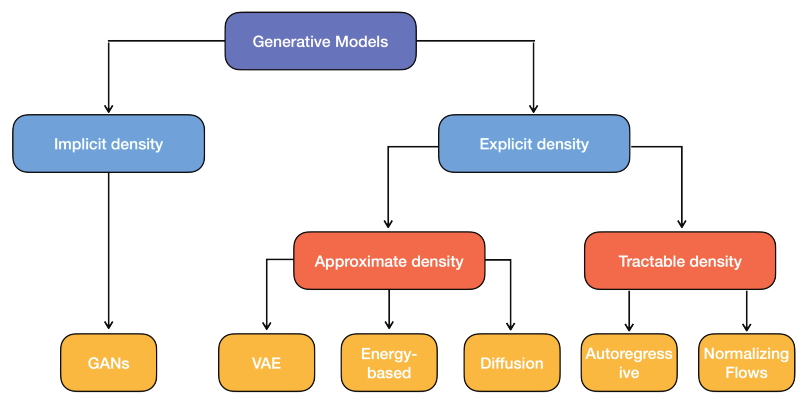
\includegraphics[width=.9\linewidth]{figures/generative-models-taxonomy.png}
	\caption{Generative Models Taxonomy}
	\label{fig:generative-models-taxonomy}
    \end{subfigure}%
    \begin{subfigure}{.4\textwidth}
	\centering
	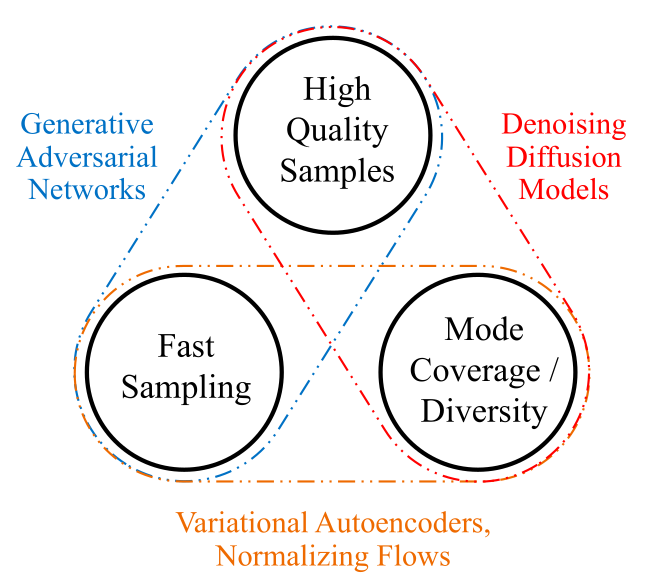
\includegraphics[width=.75\linewidth]{figures/generative-models-advantages.png}
	\caption{Generative Models Advantages}
	\label{fig:generative-models-advantages}
    \end{subfigure}
\end{figure}

\subsubsection{Generative Adversarial Networks}

Generative Adversarial Networks are a family of implicit generative algorithms that are fast to sample from.
The GAN framework is composed of two models: a \textbf{generator} $G$ with parameters $\theta$ and a \textbf{discriminator} $D$ with parameters $\varphi$.
The former learns to generate samples from the data distribution $p_\text{data}$ while the latter learns to distinguish between real and fake samples.
Therefore, contrary to single objective minimization $f : \mathcal{X} \to \R$, the optimization of a GAN is formulated as a differentiable two-player game where the generator and the discriminator aim at minimizing their own cost function as follows:
$$
\theta^* \in \arg \min_{\theta \in \Theta} \loss^\theta ( \theta, \varphi^* ) \quad \quad \quad
\varphi^* \in \arg \min_{\varphi \in \Phi} \loss^\varphi ( \theta^*, \varphi )
$$
when $\loss^\theta = -\loss^\varphi$ the game is called a \textbf{zero-sum game} and the above equation constitutes a minimax problem.

More formally, the generator receives some noise $z \sim p_z$ and computes a function $G : z \to x$ and the discriminator receives samples, some real $x \sim p_d$ and some fake obtained through $G(z)$ and computes a function $D : x \to y$.
The objective is thus
$$
\min_G \max_D \E_{x \sim p_d} \left[ \log D(x) \right] + \E_{z \sim p_z} \left[ \log (1 - D(G(z))) \right]
$$
and the losses are 
$$
\loss_G(\theta, \varphi) = \E_{z \sim p_z} \left[ \log (1 - D(G(z))) \right] \quad \quad \quad
\loss_D(\theta, \varphi) = \E_{x \sim p_d} \left[ \log D(x) \right] + \E_{z \sim p_z} \left[ \log (1 - D(G(z))) \right]
$$

The optimum solution is reached when $p_g = p_d$.
In practice, $G$ and $D$ are both neural networks and their parameters are sought after through coordinate descent with gradient based methods.

\paragraph{Conditional GAN - CGAN}

Many applications require generative model of a conditional probability distribution.
GANs can also generate samples of conditional distribution.
In
CGANs both the Generator and the Discriminator are conditioned during training by some additional information, typically the class labels

\subsubsection{Diffusion Models}

Diffusion Models work by progressively adding noise to input data and training one single model to estimate the added noise and recover the data.

More formally, Diffusion Models consider a Markov Chain with some initial distribution $p_0 = p_\text{data}$ that represents the distribution of the data and two types of transition:
\begin{itemize}
    \item The forward transition with distribution $p(x_{t+1} \mid x_t) = \mathcal{N}(x_{t+1} ; \alpha x_t, (1-\alpha^2) \mathbb{I}_d)$;
    \item The backward transition $p(x_t \mid x_{t+1})$ which can't be computed.
\end{itemize}

For the forward transition, the key insight is that the conditional $p(x_t \mid x_0)$ is also a Gaussian: $\mathcal{N}(x_t ; \alpha^t x_0, (1-\alpha^{2t}) \mathbb{I}_d)$.
Namely, as $T \to \infty$, $p(x_t \mid x_0) \to p_\text{ref} = \mathcal{N}(x ; 0, \mathbb{I}_d)$.
Therefore, for $T >>$, one can assume $p_T(x) \approx p_\text{ref}(x)$ and use this to sample $p_0$ through a method called ancestral sample, that takes advantage of the fact that:
$$
p(x_{0:T}) = p_T(x_T) \prod_{t=0}^{T-1} p(x_t \mid x_{t+1})
$$

For the backward transition, the key idea is to do some mathematical manipulation that allows us to use a neural network to approximate the distribution.

\subsection{Dimensionality Reduction}

In dimensionality reduction we want to find a lower dimension (in $\R^K$) of data (taken from $\R^D$, $D>K$) that loses as little information as possible.
This has many advantages be it for learning (less dimensions imply less parameters), visualization, compression, or even only for removing redundant features.

\paragraph{Principal Component Analysis (PCA)}

The most common algorithm for dimensionality reduction is PCA that aims at finding the linear space where the given data has most variance.
Note how increasing the variance means preserving the most information (think difference between datapoints).

More formally we want to project a set of datapoints $X = (x_1, \cdots, x_N)$ (which we'll assume are normalized) onto a linear space $L = L(u_1, \cdots, u_K)$.

Let's consider first $L = L(u)$. 
In this case, we want $\max_u \sum_{n=1}^N ||u^T x_n||^2 = \max_u u^T \Sigma u$ where $\Sigma = \frac{1}{N} \sum_{n=1}^N x_n x_n^T = \frac{1}{N} X X^T$ is the data covariance matrix.
Imposing a normalization condition to prevent that $||u|| \to \infty$, we get that to maximize the above value $u$ corresponds to the eigenvector with the largest eigenvalue $\lambda_1$ for $\Sigma$.

Note that we can now apply the same reasoning to the orthogonal projection of $L$ to extract the most information from that that was not captured by $L$.
Thus, the PCA algorithm works essentially by finding the $K$ eigenvectors of the covariance matrix $\Sigma = \frac{1}{N} X X^T$ with largest eigenvalue.

Note that the computational cost of computing the full eigenvector decomposition for a matrix of size $D \times D$ is $O(D^3)$.
If we plan to project our data onto the first $K$ principal components, then we only need $O(M D^2)$.

\section{Ethics and Fairness in ML}

Machine Learning models feed on data collected from the world and make decisions that have real world implications based on them.
Therefore, it is paramount that the bases for differentiation of these models are not unjustified or unfair as some patterns in the training represent knowledge and others represent stereotypes.
Otherwise, ML models will not only replicate but contribute to the perpetuation of discrimination.

\subsection{Fairness Criteria in Classification}

Let's consider a classification problem with input space $\mathcal{X}$, outcome variable $\mathcal{Y} = \{0,1\}$ and some random variable $A$ encoding membership status in some protected class.
We will proceed by computing some score $R = r(X)$ and make a decision $D$ according to a threshold $D = \ind[R>t]$

In order to promote fairness, $A$ must be considered as not doing so might discriminate against some classes through proxy features that are correlated with $A$.

There are three fundamental fairness criteria:
\begin{itemize}
    \item \textbf{Independence}: $R$ is independent of $A$ ($R \perp A$) - acceptance rate is the same in all groups.
    \item \textbf{Separation}: $R$ independent of $A$, conditional on $Y$ ($R \perp A \mid Y$) - misclassification rate is the same for all groups.
    \item \textbf{Sufficiency}: $Y$ independent of $A$, conditional on $R$ ($Y \perp A \mid R$) - $A$ does not provide additional information for predicting $Y$
\end{itemize}

Any of these criteria are mutually exclusive - except in degenerate cases.

\end{document}
